\documentclass[10pt,fleqn]{article}

\usepackage[english]{babel}
\usepackage[utf8x]{inputenc}
\usepackage{enumerate}
\usepackage{amsmath}
\usepackage{amssymb}
\usepackage{amsfonts} 
\usepackage{mathtools}
\usepackage{graphicx}
\usepackage{bm}
\usepackage[usenames,dvipsnames]{color}
\usepackage{todonotes}
\usepackage{dsfont}
\usepackage{hyperref}
\hypersetup{
    colorlinks,
    citecolor=black,
    filecolor=black,
    linkcolor=black,
    urlcolor=black
}
\usepackage{algorithm}
\usepackage{algorithmic}
\usepackage{appendix}
\usepackage{subcaption}
\usepackage{fancyvrb}
\usepackage{subfigure}
\usepackage{graphicx,xcolor}
\usepackage{pifont,mdframed}
\usepackage{tikz}
\usepackage{bm}
\usetikzlibrary{fit,positioning}


%
% Macros
%
\newcommand \cashort[1] { {\todo[color=yello]{#1 -- Cedric}} }
\newcommand \calong[1]  { { \todo[inline,color=yellow]{#1 -- Cedric} } }
\newcommand \gbshort[1] { {\todo[color=cyan!40]{#1 -- Guillaume}} }
\newcommand \gblong[1]  { { \todo[inline, color=cyan!40]{#1 -- Guillaume} } }
\newcommand \mgshort[1] { {\todo{#1 -- Mark}} }
\newcommand \mglong[1]  { { \todo[inline]{#1 -- Mark} } }
\newcommand \bfshort[1] { {\todo[color=green!40]{#1 -- Bryan}} }
\newcommand \bflong[1]  { { \todo[inline,color=green!40]{#1 -- Bryan} } }


% Adds a plus const to the end of a math expression
\def \pcst{+\text{const}}

% A fancy version for capital R
\def \Rcal{\mathcal{R}}

% A fancy version for r
\def \rcal{\mathbf{r}}

% Loss function / log likelihood as appropriate
\def \L{\mathcal{L}}

% KL divergence [Math Mode]
\newcommand{\kl}[2] {
	\text{KL}\left[#1||#2\right]
}

\newcommand \vecf[1] {
    \text{vec}\left(#1\right)
}

\newcommand \ent[1] {
    \text{H} \left[ #1 \right]
}

\newcommand \mut[2] {
    \text{I} \left[ #1 ; #2 \right]
}

\newcommand \dvi[2] {
    \text{D}_\text{VI} \left[ #1; #2 \right]
}

% Starts an expected value expresses [Math Mode]
\newcommand{\starte}[1] {%
	\mathbb{E}_{#1}\left[
}

% Ends an expected value expression [Math Mode]
\def \ende{\right]}

% Starts an varianc expresses [Math Mode]
\newcommand{\startv}[1] {%
	\mathbb{V}\text{ar}_{#1}\left[
}

% Ends an variance expression [Math Mode]
\def \endv{\right]}

%\newcommand \ex[2] {
%    \bigl\langle #1 \bigr\rangle_{#2}
%}
\newcommand \ex[2] {
    \mathbb{E}_{ { #2 } }\left[ #1 \right]
}
\newcommand \var[2] {
    \mathbb{V}ar_{ { #2 } }\left[ #1 \right]
}

\newcommand \halve[1] {
	\frac{#1}{2}
}

\newcommand \half {
    \halve{1}
}

\newcommand \tr { \text{tr} } 

\newcommand \T { ^\top } 

\newcommand \fixme[1] {
    {\color{red} FIXME: #1}
}

\newcommand \vv[1] { \bm #1 }

\newcommand{\mbeq}{\overset{!}{=}}

\newcommand \diag[1] { \text{diag} \left( {#1} \right) }
\newcommand \diagonal[1] { \text{diagonal} \left( {#1} \right) }

\newcommand \Ed {{ \vv{\xi}_d}}
\newcommand \Edj {{\xi_{dj}}}
\newcommand \Edk {{\xi_{dk}}}
\newcommand \AEdj {{\Lambda(\xi_{dj})}}
\newcommand \AEdk {{\Lambda(\xi_{dk})}}
\newcommand \AEd  {{ \bm{\Lambda}(\bm{\xi}_d) }}

\newcommand \Axi { { \Lambda_{\xi} } }
\newcommand \bxi { { \vv{b}_{\xi} } }
\newcommand \cxi { { c_{\xi} } }


\newcommand \wdoc      { { \vv{w}_d } }
\newcommand \wdt[0]  { { w_{dt} } }
\newcommand \wdn[0]  { { \vv{w}_{dn} } }
\newcommand \wdnt[0]  { { w_{dnt} } }
\newcommand \wdd[0]   { { \vv w_{d} } }
\newcommand \zd[0]   { { \vv z_{d} } }
\newcommand \zdn[0]  { { \vv{z}_{dn} } }
\newcommand \zdnk[0] { { z_{dnk} } }
\newcommand \zdk[0]  { { z_{dk} } }
\newcommand \thd[0]  { { \vv \theta_d } }
\newcommand \thdk[0] { { \theta_{dk} } }
\newcommand \thdj[0] { { \theta_{dj} } }
\newcommand \epow[1] { { e^{#1} } }
\newcommand \pkt     { { \phi_{kt}  } }
\newcommand \pk      { { \vv \phi_k } }
\newcommand \lmd     { { \vv \lambda_d } }
\newcommand \lmdk    { { \lambda_{dk} } }
\newcommand \xd      { { \vv x_d } }
\newcommand \atxd     { A ^\top \bm x_d}
\newcommand \axd     { A\bm x_d}
\newcommand \tsq      { { \tau^2 } }
\newcommand \ssq      { { \sigma^2 } }
\newcommand \tmsq     { { \tau^{-2} } }
\newcommand \asq      { { \alpha^2 } }
\newcommand \amsq     { { \alpha^{-2} } }
\newcommand \sgsq     { { \sigma^2 } }
\newcommand \xvec     { { \vv{x} } }
\newcommand \omk      { { \bm \omega _k } }
\newcommand \omkt     { { \omega_{kt} } }
\newcommand \oma     { { \Omega_A } }
\newcommand \gdn      { { \vv{\gamma}_{dn} } }
\newcommand \gdnk     { { \gamma_{dnk} } }
\newcommand \gdk      { { \gamma_{dk} } }
\newcommand \isigt   { { \Sigma^{-1}_{\bm \theta} } }




\newcommand \halfSig { \frac{1}{2\sigma^2} }

\newcommand \nor[2]   { \mathcal{N} \left( {#1}, {#2} \right) }
\newcommand \nord[3]   { \mathcal{N}_{#1} \left( {#2}, {#3} \right) }
\newcommand \mnor[3]  { \mathcal{N} \left(#1, #2, #3\right) }
\newcommand \norp[3]  { \mathcal{N} \left(#1; #2, #3\right) }
\newcommand \mnorp[4] { \mathcal{N} \left(#1; #2, #3, #4\right) }
\newcommand \mul[1]   { \mathcal{M} \left( {#1} \right) }
\newcommand \muln[2]  { \mathcal{M} \left( {#1},{#2} \right) }
\newcommand \dir[1]   { \mathcal{D} \left( {#1} \right) }
\newcommand \pois[1]  { \mathcal{P} \left( {#1} \right) }
\newcommand \gp[2]    { \mathcal{GP} \left( {#1}, #2 \right) }
\newcommand \dir[1]   { \mathcal{D} \left( {#1} \right) }
\newcommand \gam[2]   { \mathcal{G} \left( {#1}, {#2} \right) }
\newcommand \beta[1]  { \mathcal{B}eta \left( {#1}, {#2} \right) }

\newcommand \lne[1]  { { \ln \left( 1 + e^{ #1 } \right) } }
\newcommand \Tr[1]   { \tr \left(  {#1}  \right) }

\newcommand \roud  { \vv{\rho}_{d}  }
\newcommand \rodk { \rho_{dk} }

\newcommand \exA[1]  { \ex{#1}{q(A)} }
\newcommand \exV[1]  { \ex{#1}{q(V)} }
\newcommand \exT[1]  { \ex{#1}{q(\Theta)} }
\newcommand \extd[1] { \ex{#1}{q(\thd)} }
\newcommand \exTV[1] { \ex{#1}{q(\Theta)q(V)} }

\newcommand \Real[0]  { { \mathbb{R} } }
\newcommand \VReal[1] { { \mathbb{R}^{#1} } }
\newcommand \MReal[2] { { \mathbb{R}^{#1 \times #2} } }
\newcommand \Nat[0]  { { \mathbb{N} } }
\newcommand \VNat[1] { { \mathbb{N}^{#1} } }
\newcommand \MNat[2] { { \mathbb{N}^{#1 \times #2} } }

\newcommand \inv[1] { {#1}^{-1} }
\newcommand \invb[1] { \inv{\left( #1 \right)} }

\newcommand \cn { \textsuperscript{\texttt{[{\color{blue}Citation Needed}]}} }

\newcommand \const { { \text{c} } }

\providecommand \floor [1] { \left \lfloor #1 \right \rfloor }
\providecommand \ceil [1] { \left \lceil #1 \right \rceil }


\newcommand \vt[2] { { #1^{(#2)} } }

\newcommand \hashtag[1] { { \ttfamily \##1 } }

\newcommand \mvy  { \vv{m}_{\vv{y}} }
\newcommand \sigvy { { S_Y } }

\newcommand \mmy  { M_Y      }
\newcommand \md   { \vv{m}_d }
\newcommand \phin { \vv{\phi}_n }
\newcommand \isigma { { \inv{\Sigma} } }

\newcommand \sigv     { { \Sigma_V } }
\newcommand \isigv     { { \Sigma^{-1}_V } }

\newcommand \sigy { { \Sigma_Y } }
\newcommand \isigy { { \Sigma_{-1}_Y } }


\newcommand \omy  { { \Omega_Y } }
\newcommand \iomy { { \inv{\Omega_Y} } }

\newcommand \siga     { { \Sigma_A } }
\newcommand \isiga     { { \Sigma^{-1}_A } }
\newcommand \diagv { { \diag{\nu_1,\ldots,\nu_P} } }

\newcommand \ma { \vv{m}_a }
\newcommand \my { \vv{m}_y }

\newcommand \VoU { V \otimes U }

\newcommand \one { \mathbb{1} }
%\newcommand \one  {{  \mathds{1} }}

\newcommand \lse { \text{lse} }
%\newcommand \lse[0] { \mathrm{lse} }

% Conditional independence 
\def\ci{\perp\!\!\!\perp} % from Wikipedia



% ------ For the eval section

% Multinomial PDF [Math Mode]
% params: 1 - the variable
%         2 - the value
%         3 - the state indicator (e.g. k for a distro with K values)
%         4 - any additional subscript
\newcommand{\mpdf}[4] {
	\prod_{#3} {#1}_{{#4} {#3}} ^ {#2}
}

% Dirichlet PDF [Math Mode]
% params: 1 - the variable
%         2 - the hyper-parameter
%         3 - the state indicator (e.g. k for a distro with K values)
%         4 - any additional subscript
\newcommand{\dpdf}[4] {
	\frac{1}{B({#2})} \prod_{#3} {#1}_{{#4} {#3}} ^ {({#2}_{#3} - 1)}
}

% To simplify the sampling equations, this is indicates
% that the given value has had datapoint "m" stripped out
%
\newcommand{\lm}[1] {
	#1^{\setminus m}
}

\newcommand \model[0] {
    \mathcal{M}
}

\newcommand \perplexity[1] {
    \mathcal{P} \left( { #1 } \right)
}

\newcommand \WTrain {
    \mathcal{W}^{(t)}
}

\newcommand \WQuery {
    \mathcal{W}^{(q)}
}

\newcommand \oneover[1] {
    \frac{1}{ {#1} }
}

\newcommand \samp[1] {
    { #1 }^{(s)}
}

\newcommand \etd[0] {
    \vv{\eta}_d
}

\begin{document}



\subsection{Inference Strategies}
LDA has proved to be a very popular algorithm in practice, with deployments in Yahoo\cite{Ahmed2011a}, Last.fm\footnote{\url{http://mir-in-action.blogspot.co.uk/2011/04/algorithms-on-hadoop.html}} and others. Considerable effort has been focused on the best possible implementations of LDA for batch, online and distributed computation.

In the following we will use the notation $n_{dkt}$ to indicate the number of instances of term $t$ assigned to topic $k$ in document $d$, and will use a dot to indicate when a summation has occurred, such that $n_{\cdot k t} = \sum_d n_{dkt}$.

% Do this in the intro to admixtures.
%In the following presentation we will assume that there  are $D$ documents with a vocabularly of $T$ words described by $K$ topics, indexed by $d,t$ and $k$ respectively. 

%https://github.com/shravanmn/Yahoo_LDA
%http://www.slideshare.net/MarkLevy/algorithms-on-hadoop-at-lastfm

The initial implementation of LDA presented in \cite{BleiNgJordan2003} employed a variational inference algorithm using a fully-factorized variational posterior

While one could also derive a Gibbs sampler, with separate posteriors for $\thd$, $\zdnk$ and $\pk$ \cite{Pritchard2000} the strong dependencies between parameters typically impede convergence\cite{CasellaRobert1999}. Therefore \cite{Griffiths2004} a Rao-Blackwellised sampler was derived by marginalising out $\thd$ and $\Phi$:

Due to conjugacy, collapsing out $\pk$ and $\thd$ leads to a product of P\:olya distributions as described in section\begin{align}
p(W,Z|\vv{\alpha},\vv{\beta}) = \prod_d \frac{B(\vv{n}^{(d)} + \vv{\alpha})}{B(\vv{\alpha})} \prod_k \frac{B(\vv{n}^{(k)} + \vv{\beta})}{B(\vv{\beta})}
\end{align}
where the document-topic count vector $\vv{n}^{(d)} = \{ n_{dk\cdot} \}_{k=1}^K$ and $\vv{n}^{(k)} = \{ n_{\cdot kt} \}_{t=1}^T$. From this we can derive (see \cite{Heinrich2005} for a fully worked out example) the posterior over topics
\begin{align}
p(z_{dn} = k | \vv{z}_{d}^{\setminus dn}, \vv{w}_d)
\propto
\left(n_{dk\cdot}^{\setminus dn} + \alpha_k \right)
\frac{n_{\cdot kt}^{\setminus dn} + \beta_t}{\sum_v n_{\cdot kv}^{\setminus dn} + \beta_v}
\end{align}
which takes on the familiar Bayesian form of a product of a prior (over topics) and a likelihood. This was compared to the uncollapsed sampler of \cite{Pritchard2000} in \cite{Newman2009} and exhibited much faster convergence on the standard NIPS dataset

One can also take the same approach with variational inference. As with a Gibbs sampler, one simply marginalizes out the distribution over topics and vocabularies, following posterior\cite{Teh2007}:
\begin{equation}
q(\zdnk) \propto \exp\left(\ex{
    \ln (n_{dk\cdot}^{\setminus dn} + \alpha_k ) 
    + \ln (n_{\cdot kt}^{\setminus dn} + \beta_t)
    - \ln (\sum_v n_{\cdot kv}^{\setminus dn} + \beta_v)}{q(Z^{\setminus dn})}
\right)
\end{equation}
In this update, the random variables over which the expectation is taken are the counts $n_{dnt}$, which are the sum of a large number of Bernoulli random variables, which can in turn be approximated by a Gaussian. The expected value in turn can be approximated by a second order Taylor approximation around the true mean (an approach known as the ``delta method"\cite{Wang2013}), such that
\begin{align}
\ex{\ln (n_{dk\cdot}^{\setminus dn} + \alpha_k )}{\hat{q}} 
\approx 
\ln (\ex{n_{dk\cdot}^{\setminus dn}}{\hat{q}} + \alpha_k ) - \frac{\var{n_{dk\cdot}^{\setminus dn}}{\hat{q}}}{2\left( \ex{n_{dk\cdot}^{\setminus dn}}{\hat{q}} + \alpha_k \right)^2}
\end{align}
where $\ex{n_{dk\cdot}^{\setminus dn}}{\hat{q}} = \sum_{i \neq n} z_{dik}$ and $\var{n_{dk\cdot}^{\setminus dn}}{\hat{q}} = \sum_{i \neq n} z_{dik}(1 - z_{dik})$. This algorithm is known as LDA/CVB. A simpler variant exists which using a zero-th order Taylor approximation, and so lacks the variance term, which is known as LDA/CVB0.\cite{Asuncion2012} 


\begin{figure}
  \centering
    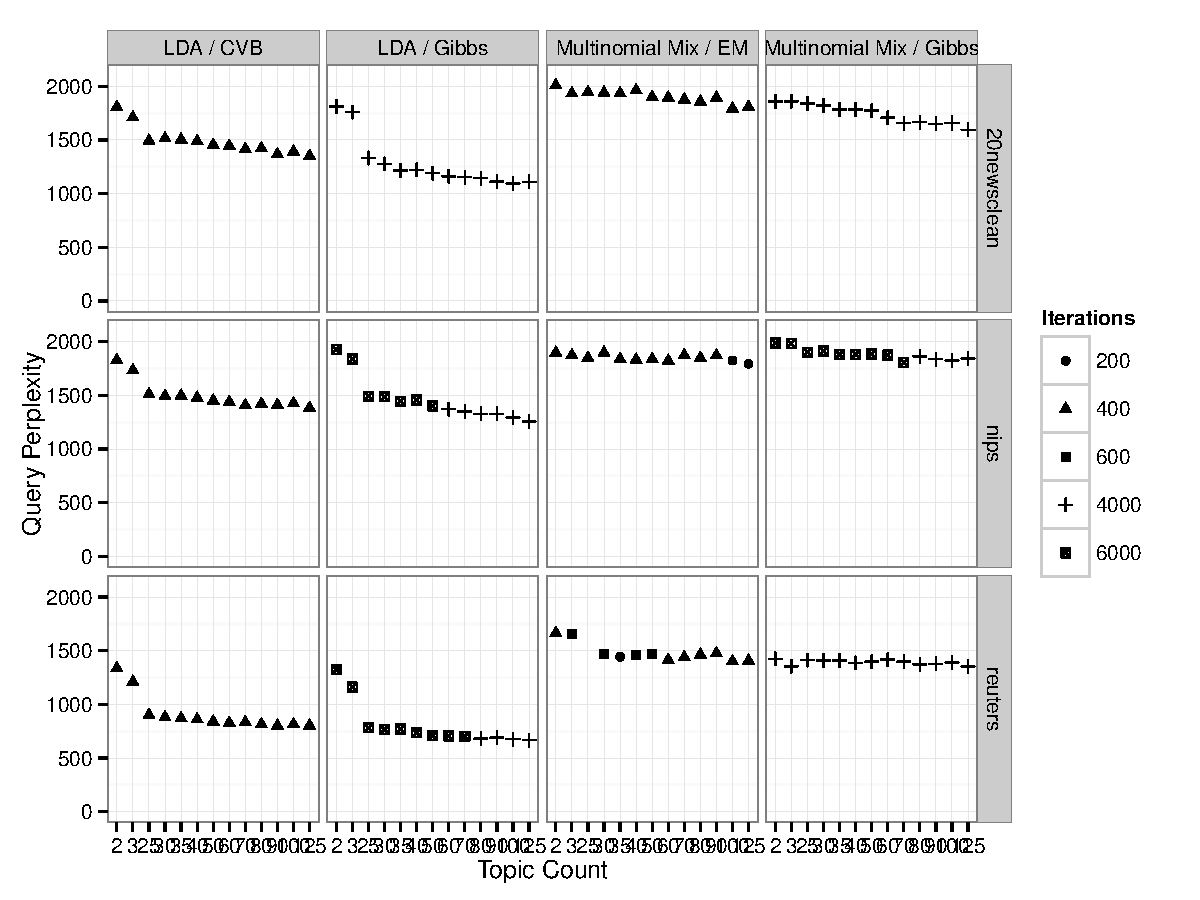
\includegraphics[width=\textwidth]{plots/results-2013-03-18-bw.pdf}
  \caption{Perplexity results for LDA and a mixture of multinomials ("MoM") implemented using Gibbs sampler and EM in the case of the mixture, and collapsed variational inference in the case of LDA. The three datasets are Reuters, NIPS, and four distinct newsgroups from the 20News dataset. The number of iterations (including burn-in for samplers) is also shown.}
  \label{fig:nip-reuters-20news-tests}
\end{figure}


A deficiency of collapsed variational LDA however versus a Gibbs sampler, and even fully-factorised variational inference, it requires the storage of all topic-assignments $\zdnk$ in addition to the counts $n_{dk\cdot}$ and $n_{\cdot kt}$ making it the most memory intensive of all the methods described.

In \cite{Asuncion2012} all four methods, LDA/VB, LDA/Gibbs, LDA/CVB and LDA/CVB0, and a further inference algorithm based on MAP-estimation were compared against each other on several datasets using a common evaluation metric known as perplexity (see section \ref{sec:eval}). LDA/VB performed worst of all, with LDA/Gibbs and LDA/CVB having comparable performance, and LDA/CVB0 having best performance of all. This is a strange result, as LDA/CVB0 involves an ostensibly \emph{worse} approximation of the expectation over LDA/CVB. 

An explanation for this was given in\cite{Sato2012} who showed that the terms in the LDA/CVB0 update can be understood as optimizing the $\alpha$-divergence\cite{Minka2005}, with different values of $\alpha$ for each term. The $\alpha$-divergence is a generalization of the KL-divergence that variational Bayes minimizes, and optimizing it is known as power EP. An EP implementation of LDA has also been derived in \cite{Minka2002}

Regarding the performance of LDA/CVB compared to a collapsed Gibbs sampler, in our experiments (see figure \ref{fig:nip-reuters-20news-tests}) a Gibbs sampler always outperformed LDA/CVB, albeit by a small margin.

One can relate the Gibbs procedure to the batch variational procedure by means of two approximations. The variational posterior over a topic for a single word is:
\begin{align}
q(z_{dnk}) \propto \exp(\ex{\ln \theta_{dk}}{q})\exp(\ex{\ln \phi_{k,w_{dn}}}{q})
\label{eqn:fac-var-zdnk}
\end{align}
where $\ex{\ln \theta_{dk}}{q} = \psi(\gamma_{dk}) - \psi(\sum_j \gamma_{dj})$ and $\vv{\gamma}_d$ is the parameter of the variational posterior over $\thd$. If one substitutes the updates for the posteriors over $\pk$ and $\thd$ into \eqref{eqn:fac-var-zdnk} and then approximates $\exp(\psi(n)) \approx n - \half$ (which holds for large positive numbers) the posterior becomes:
\begin{align}
q(z_{dnk}) \approxpropto \left(n_{dk\cdot} + \alpha - \half\right) \cdot \frac{n_{\cdot k w_{dn}} + \beta_{w_{dn}} - \half}{\sum_t n_{\cdot k t} + \beta_t - \half}
\end{align}
This illustrates that the main difference between the Gibbs sampler and the fully-factorised variational inference is that the variational approach is less regularlised (due to the $-\half$ term), and that the counts $n_{dkt}$ are only updated after all documents have been processed, rather than after each individual token as happens with the Gibbs sampler: it also suggests that the performance of the fully-factorized VB could be brought closer to the Gibbs approach through the use of stochastic gradient ascent\cite{Hoffman2012} , where the counts are updated after every document.

%Whilst discussing LDA/CVB, it should not noted that an alternative approach to collapsing out terms was taken in \cite{Hensman2012}, where the parameters were marginalized \emph{after} applying the variational bound instead of before. On a small dataset they demonstrated faster convergence relative to LDA/VB, but did not compare to LDA/CVB directly.


\subsection*{Scaling to Large Datasets}
The issue of how to scale LDA to large datasets has been actively researched. In the variational case, the natural choice is the use of stochastic gradient ascent\cite{Bottou2004}\cite{Bottou2008} to infer each document's topic-distribution, and then immediately use it to perform a gradient update on the vocabulary\cite{Hoffman2010}\footnote{In practice ``mini-batches" of documents are used to minimise the variance}. Performance can be further improved by using Gibbs sampling to get a sparse estimate of the topic distribution, permitting sparse calculations throughout\cite{Mimno2012a}.

The LDA/CVB, algorithm, with just one parameter, does not fit the ``local-global" split exploited by stochastic methods, particularly as the previous value of $\zdnk$ is required to estimate terms such as $\ex{n_{dk\cdot}^{\setminus dn}}{\hat{q}}$. Attempts to scale this\cite{Boyles2013} simply ignore the subtraction and treat counts as random variables updated using gradient steps in the Online EM framework\cite{Cappe2009}. This reduces the memory requirements of LDA/CVB, but not its runtime.
%\fixme{Need to read Sparse Online Topic Models\cite{Zhang2013}}

Significant effort has also been expended on making Gibbs sampling scale to large datasets. Many of these algorithmic improvements are described in \cite{Yao2009} which builds on results in \cite{Porteous2008}. The most notable is to re-write the sampling distribution as

\newcommand \nodn { { ^{\setminus dn } } }

\begin{align}
\begin{split}
p(z_dn = k | \vv{z}_{d}^{\setminus dn}, w_{dn}=t) & \propto \frac{\alpha_k \beta_t}{n_{\cdot k \cdot}\nodn + \sum_v \beta_v} \\
& + n_{dk\cdot}\nodn \frac{n_{\cdot kt}\nodn + \beta_t}{n_{\cdot k \cdot}\nodn + \sum_v \beta_v} \\
& + \frac{n_{dk\cdot}\nodn n_{d\cdot t}\nodn}{n_{\cdot k \cdot}\nodn + \sum_v \beta_v}
\end{split}
\end{align}
While ostensibly more complicated, the second and third summands are sparse, and can be stored efficiently, while the first term, which is dense, is trivially changed after each update as only the denominator changes.
%\fixme{See also Fast collapsed gibbs sampling for latent dirichlet allocation. In Proceedings of the ACM SIGKDD International Conference on Knowledge Discovery and Data Mining, pages 569–577, 2008.}

Distributed computation has also been a subject of particular interest. Since $M$ machines have $2^M$ possible links, it unfeasible for machines should communicate, so the problem is to infer a model where the $D$ topics have been partitioned across $M$ machines which can operate independently.

The trivial solution is to implement an uncollapsed Gibbs sampler: topic assignments are conditionally independent given $\thd$ and $\pk$, so one can distributed the task of estimating $z_{dn} | \thd, \Phi$ across all machines, and at the end of an iteration use the results to update $\Theta$ and $\Phi$ globally. However uncollapsed Gibbs samplers typically exhibit poor mixing.

AD-LDA\cite{Newman2009} is a distributed, collapsed Gibbs sampling algorithm. The three sufficient statistics of a collapsed Gibbs sampler are the counts $n_{dk\cdot}$, $n_{\cdot k \cdot}$ and $n_{\cdot k t}$. A machine $m$ will know the first for the documents it stores, but will not be aware of the other two. AD-LDA, simply ignores this. At the start of each iteration, the full counts $n_{\cdot kt}$ are broadcast to all machines, and then they proceed, using their local copies of these counts, to draw samples and so create updated counts. These are then summed together at the end of the iteration, ready for the start of the next. 

The intuition behind this approximation is that due to the large number of words, the number of word-topics changed by other machines $m' \neq m$ in a single iteration will have a negligible effect on the probabilities of topic assignment on machine $m$, and so the presence of such ``stale" counts on a machine $m$ disconnected from all machines $m' \neq m$ will be negligible.

This approach can be formalised by modelling each machine as having its own noisy sample of the topic-word counts sampled from some global distribution, which leads to naturally leads to a hierarchical model. In such a model each machine's vocabulary distributions are sampled from global vocabularies, such that topic-assignments can be considered conditionally independent given these vocabularies.
\begin{align}
\alpha^{(m)} & \sim \gam{a}{b} &
\vv{\theta}_d^{(m)} & \sim \dir{\alpha^{(m)}} &
\vv{\psi}_k^{(m)} & \sim \dir{\gamma} \\
\beta_k & \sim \gam{c}{d} &
z_{dn}^{(m)} & \sim \muln{\vv{\theta}_d^{(m)}}{1} &
\vv{\phi}_k^{(m)} & \sim \dir{\beta_k \vv{\psi}_k} \\
& &
& &
w_{dn}^{(m)} & \sim \muln{\vv{\phi}_{z_{dn}^{(m)}}^{(m)}}{1}
\end{align}

This approach defines a valid probabilistic model which can be decomposed across machines, but identifiability remains an issue i.e. topic \#1 on one machine may correspond to a topic \#7, say, on another. One can simply ignore this, and hope the model converges, but an improvement is to consider a greedy strategy where one machine's topics are considered the gold standard, and each subsequent machine's topics are matched to those topics using KL-divergence. Where no acceptably close match occurs, one can add a new topic, allowing $K$ could change between runs. 

In practice\cite{Newman2009}, the reported convergence and predictive likelihood was broadly similar between the approximate and hierarchical distributed samplers using the same reconciliation strategy, and inference did succeed, albeit slowly, if one ignored identifiability. Both models still showed worse convergence on small datasets than the non-distributed batch model however.

To avoid identifiability issues, and the use of approximations or hierarchies, counts need to be broadcast across all machines immediately. This is achieved by creating a shared, high-speed parameter stored, a ``blackboard server"\cite{Smola2010} which all machines can access: this particularly works if no machines try to access the same field at the same time. This is true of document-topic counts, $n_{dk}$, if each document's words are on a single server. The counts $n_{\cdot k \cdot}$ and $n_{\cdot k t}$ are more problematic but if accessed only at the start and end of a document, contention is reduced. 

A further advantage of this model is that all machines can iterate to convergence independently, instead of pausing at the end of each iteration to reconcile counts.

With respect to large-scale inference among correlated topic models, if one augments the model with an auxiliary variable $\lambda_{dk}$ one can re-write the sampling distribution over the unnormalised topic-strength $\eta_{dk}$ as:
\begin{align}
p(\eta_{dk} | \vv{\eta}_{d\setminus k}) & = \frac{(e^{\rho_{dk}})^{n_{dk\cdot}}}{(1 + e^{\rho_{dk}})^{n_{d\cdot\cdot}}} \qquad\qquad\qquad\text{where }\rho_{dk} = \eta_{dk} - \ln\left(\sum_{j \neq k} \eta_{dj}\right) \\
&= \frac{1}{2^{n_{d\cdot\cdot}}}
e^{\kappa_{dk} \rho_{dk}}
\int_0^\infty e^{-\halve{\lambda_{dk} (\rho_{dk})^2}} p(\lambda_{dk}|n_{d\cdot\cdot},0) d\lambda_{dk} 
\end{align}
where $\kappa_{dk} = n_{dk\cdot} - \halve{n_{d\cdot\cdot}}$ and $\lambda_{dk}$ has a Polygamma distribution. With this representation one can derive an exact Gibbs step, instead of resorting to the more usual approach of rejection sampling. Combined with certain approximation steps, this leads to rapid inference\cite{Chen2013}. To use this in a distributed environment one simply uses hierarchical priors as in AD-LDA: specifically the topic strength vectors $\vv{\eta}_d$ for each document $d$ are conditionally independent of one another given the $\mathcal{NIW}\left(\vv{\mu}, \rho, \kappa, \Sigma\right)$ prior. The per-token topic assignments need the global $n_{\cdot k t}$ counts, and these are made available via a blackboard server.

\subsection*{Inference of Hyperparameters}
In its original presentation\cite{BleiNgJordan2003} the parameters of the prior distributions on topics and vocabularies ($\vv{\alpha}$ and $\vv{\beta}$ respectively), were inferred using a fast Newton-Raphson update procedure described in \cite{Minka2000}:

\begin{align}
\alpha_k = \frac{\alpha_k \left( \left(\sum_d \Psi(n_{dk\cdot} + \alpha_k \right) - D \Psi (\alpha_k)\right)}{\left(\sum_d  \Psi(\sum_k n_{dk\cdot} + \alpha_k \right) - D \Psi (\sum_k \alpha_k)}
\end{align}

where $\Psi(\cdot)$ is the digamma function This should be iteratively evaluated till convergence. The update for $\beta_t$ follows similarly. This method is not particularly stable however, and is very sensitive to the choice of initial estimate.

Despite this, many implementors in the literature choose to use fixed, symmetric hyper-parameters, typically following advice in \cite{Griffiths2004} to set $\alpha_k = \frac{50}{K}$ and $\beta_t=0.1$. 

Note that symmetric LDA hyperparameter values are coupled, smaller values of $\alpha$ encourage sparser topic assignments, which in turn require either denser topic-specific vocabularies (affecting $\beta$) or a larger number of topics, in order to reconstruct the original document.


%S too can be learnt in a variational framework, by a modification of the above update\cite{Heinrich2005}:
%
%\begin{align}
%\alpha = \frac{\alpha \left( \left(\sum_d \sum_k \Psi(n_{dk\cdot} + \alpha_k \right) - DK \Psi (\alpha)\right)}{K \left( \left(\sum_d  \Psi(\sum_k n_{dk\cdot} + \alpha \right) - D \Psi (K \alpha)\right)}
%\end{align}

Despite this widespread use of symmetric, fixed, hyperparameters, experiments have shown\cite{Wallach2009a} that while learning the prior over vocabulary has no significant effect on performance, substantial improvements can be gained by learning the prior over topics. Moreover, a useful side-effect of this procedure is that stop-words are all captured by the most likely topic making interpretation of other topics much easier. The suggested approach os a hierarchical model, where Gamma-Dirichlet hyper-priors was placed over the contentration and base-measure of the Dirichlet priors, enabling a Gibbs sampling scheme to be used to learn the priors.



% ---- Gibbs optimisations ----




% ---- Other approaches ----



\bibliographystyle{plain}
\bibliography{/Users/bryanfeeney/Documents/library.bib}

\end{document}

